\section{Neuronky}
\subsection{Hloubka sítě, výpočet, princip}

Hloubka neuronové sítě definuje počet vrstev neuronů, které nn obsahuje.

\subsection{Princip konvolučních sítí}
Konvoluční neuronové sítě narozdíl od ostatních přivádí jiné vrstvy než plně propojené. Tyto sítě jsou založeny na kombinování různých typů vrstev, plně
propojených, konvolučních, max-pooling. Můžou se používat pro různé dimenze dat 1D pro time-series nebo zpracování hlasu, 2D pro zpracování obrazu, 3D pro data z
MRI nebo CT.\\
\subsubsection{Konvoluční vrstva}
Vrstva je založena na konvoluci vstupních dat s konvolučním kernelem. Tento kernel je reprzentován maticí vah, která se posouvá po vstupních datech. Pomocí těchto
kernelů se provádí často operace pro zjednodušení vstupních dat, například detekce hran v obraze. Konvoluce jako taková je matematická operace, která funguje na 
pricipu násobení části vstupu maticí vah a součet výsledku těchto součinů. Pokud máme matici X vstupu 3x3 a kernel K velikosti 3x3 pak bude výsledek konvoluce následující:\\
\begin{align*}
    c = x_{00}\cdot k_{00} + x_{01}\cdot k_{01} + x_{02}\cdot k_{02} + ... + x_{33}\cdot k_{33}
\end{align*}
Vedlejší efekt konvoluce je ten, že zmenšuje vstup a to podle velikosti konvolučního kernelu. Z toho důvodu se často přidává ohraničení 0 tak aby vstupní data
zůstala stejné velikosti.\\
\begin{figure}[ht]
    \centering
    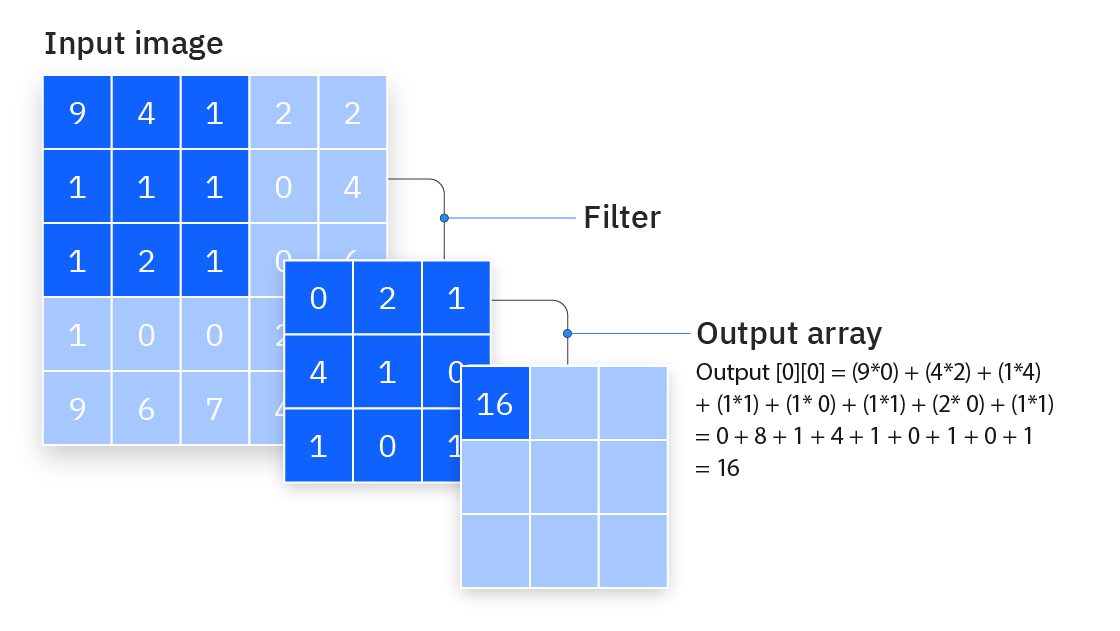
\includegraphics[scale = 0.25]{images/iclh-diagram-convolutional-neural-networks.png}
\end{figure}
\subsubsection{Max Pooling vrstva}
Její účel je zmenšení vstupu pro jednodušší zpracování a zárovenň zachování nejdůležitější informace z oblasti. Stejně jako koncvoluční vrstva používá kernel
pro procházení vstupu. Avšak místo sumy bere pouze největší hodnotu z oblasti přes kterou se kernel posouvá.\\
\begin{figure}[ht]
    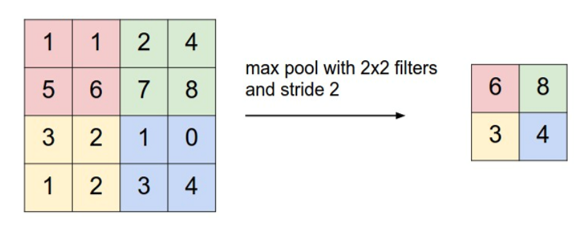
\includegraphics[scale=0.7]{images/MaxPooling.png}
\end{figure}

\subsubsection{Flatten vrstrva}
Používá se po dokončení práce konvolučních a max pooling vrstev pro transformaci dat z matice do vektoru aby mohly být data zpracovány plně propojenými vrstvami. 

\subsubsection{Augmentace dat}
Používá se pro zvýšení různorodosti datasetu. Přidává další data pomocí transformací dat známých.
U obrazu sem patří posuny, rotace, zrcadlení, úpravy kontrastu, jasu, atd. U zvuku například přidání šumu do pozadí, posun tóniny.

\subsubsection{Transfer learning}
Využití toho, že již existují velké sítě, které jsou již natrénované na obřích datasetech a my si doděláme k tomuto modelu jenom klasifikátor.

\subsection{Rekurentní neuronky}
Rekurentní nn používají cykly a faktorem je zde i čas.
Zpracovávají sekvence dat na sekvence výstupů. Narozdíl od klasický NN mají paměť, jejich vnitřní stav označovaný \(h(t)\) je použit pro operaci s dalším vstupem.\\
\begin{figure}[ht]
    \centering
    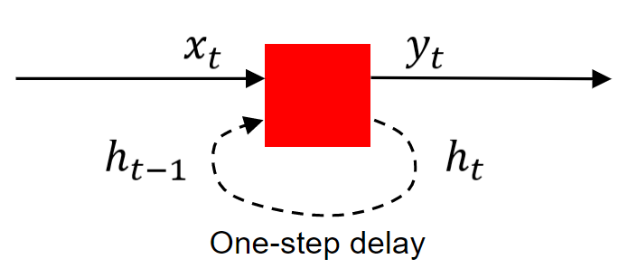
\includegraphics[scale = 0.5]{images/RNN.png}
\end{figure}

\subsubsection{LSTM}
Long Short Term Memory. Pokročilá varianta RNN. Má mnohem složitěší buňku, která je založena na používání bran(gates) pro kontrolu toku informací. LSTM buňka má
4 stavy zpracování:
\begin{enumerate}
    \item Zapomene nepotřebnou historii
    \item Uloží relevantní části nové informace
    \item Pomocí předchozích 2 kroků aktualizuje vnitřní stav
    \item Generuje výstup
\end{enumerate}
